\documentclass[a4paper,12pt]{article}
\usepackage[utf8]{inputenc}
\usepackage[top=2cm,bottom=2.54cm,left=2.54cm,right=2.54cm]{geometry}
\usepackage[namelimits]{amsmath} 
\usepackage{amssymb}             
\usepackage{amsfonts}            
\usepackage{mathrsfs}            
\usepackage{graphicx}
\usepackage{subfigure}
\usepackage{multirow}
\usepackage{listings}
\usepackage{diagbox}
\usepackage{slashbox}
\lstset{language=Matlab}
\lstset{breaklines}
\lstset{extendedchars=false}

\title{Fintech545 Homework 2}
\author{qw112 Qiyu Wu}
\date{}

\begin{document}
\maketitle  
\subsection*{Question 1.Exponentially Weighted Covariance Matrix}
For the question, there are steps that have been done to make the weighted covariance matrix, assume the weight $\lambda$ has been known:
\begin{itemize}
    \item Read csv file data and adjust index and column name for the dataset;
    \item Generate weights for each time point (60 time points in total);
    \item Applied exponentially weighted covariance formula to generate 101$\times$101 covariance matrix;
\end{itemize}
After finishing all the above steps, we can get one covariance matrix for each specific $\lambda$. Then, we can investigate the relationship between the explanationary power of PCA and the $\lambda$ value. 
\begin{center}
    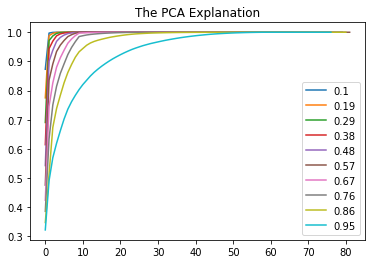
\includegraphics[width=10cm]{Q1.png}
\end{center}
\textbf{Conclusion:}
\begin{itemize}
    \item \textbf{Findings:} For the same n value, when $\lambda$ approaches to 0, the less explanationary power will be.
    \item \textbf{Reasons:} Exponentially Weighed means that weights put on the time near to the current time, which also means the smaller time lag. So, when $\lambda$ become smaller, it means that people put more consideration on the older time. In this way, We need more time point to generate high explanationary power in the PCA method.
\end{itemize}

\newpage
\subsection*{Question 2. Methods to Deal with Non-Positive Semidefinite Matrix}
Within the question, we try to use near\_psd() and Higham method to fix a non-PSD Matrix. According to the new eigenvalue based on the fixed matrix, the covariance matrix is now PSD. Then, we would like to know more to compare the  
\begin{figure}[!htbp]
    \subfigure{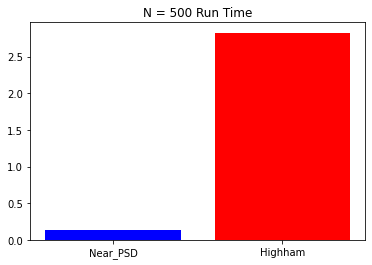
\includegraphics[width=8cm]{500_run.png}}
    \subfigure{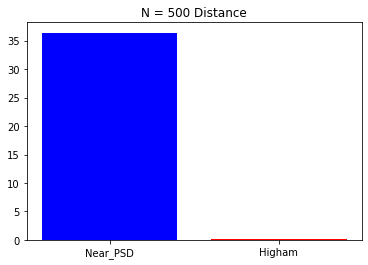
\includegraphics[width=8cm]{500_dis.png}}\\
    \subfigure{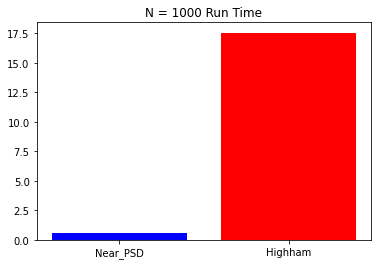
\includegraphics[width=8cm]{1000_run.png}}
    \subfigure{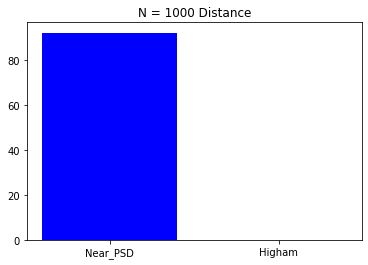
\includegraphics[width=8cm]{1000_dis.png}}\\
    \subfigure{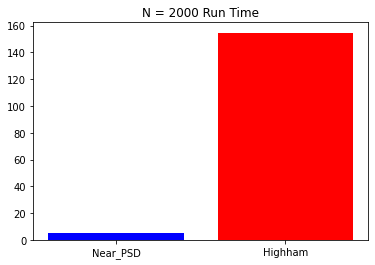
\includegraphics[width=8cm]{2000_run.png}}
    \subfigure{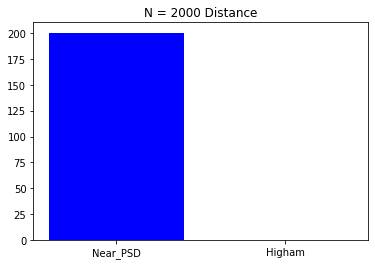
\includegraphics[width=8cm]{2000_dis.png}}\\
\end{figure}

\textbf{Conclusion:}
\begin{itemize}
    \item From the general point of view, out of the accuracy needs, we need use the Higham's method to adjust non-psd matrix. It has a small distance difference under all cases.
    \item To improve the run time efficiency, the Near\_PSD would be a better choice. It is consistently fast even when N is larger. 
\end{itemize}

\newpage
\subsection*{Question 3. Principle Component Analysis}
\subsubsection*{Construct 4 Covariance Matrix}
Here are Combinations about my construction:
\begin{itemize}
    \item Pearson Correlation \& Pearson Variance
    \item Exponentially Weighted Correlation \& Exponentially Weighted Variance
    \item Pearson Correlation \& Exponentially Weighted Variance
    \item Exponentially Weighed Correlation \& Pearson variance
\end{itemize}
According to the 4 Covariance Matrix, We perform analysis about the 4 covariance matrix from 4 perspectives: Direct Simulation, and $100\%$, 75\%, 50\% PCA. \\
\subsection*{Visutalization Analysis}
Here are visualization about their run time and distane between real covariance matrix and covariance matrix gain from simulation. Since the difference of distance between different PCA explanation requirements, we made a table for it.\\

\begin{figure}[!htbp]
    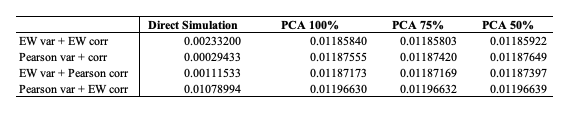
\includegraphics[width=15cm]{pca.png}
    \caption{Distance Table of Covariance Matrix}
\end{figure}

\begin{figure}
    \subfigure{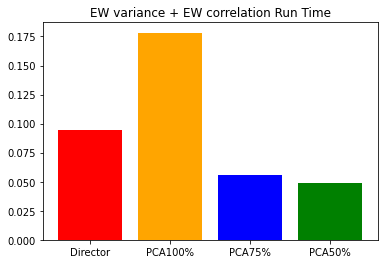
\includegraphics[width=8cm]{EE_run.png}}
    \subfigure{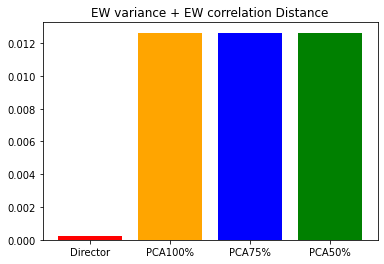
\includegraphics[width=8cm]{EE_dist.png}}\\
    \subfigure{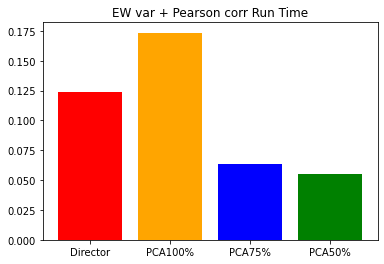
\includegraphics[width=8cm]{EP_run.png}}
    \subfigure{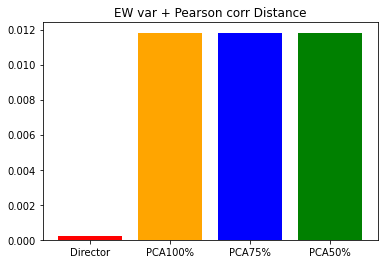
\includegraphics[width=8cm]{EP_dis.png}}\\
    \subfigure{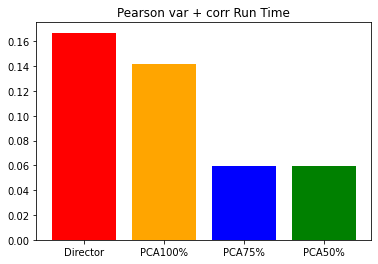
\includegraphics[width=8cm]{PP_run.png}}
    \subfigure{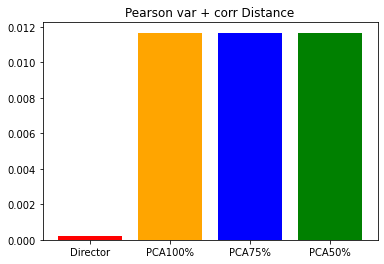
\includegraphics[width=8cm]{PP_dis.png}}\\
    \subfigure{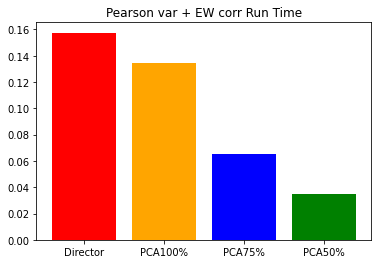
\includegraphics[width=8cm]{PE_run.png}}
    \subfigure{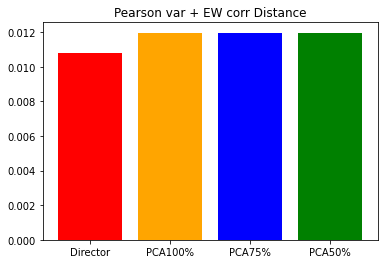
\includegraphics[width=8cm]{PE_dis.png}}\\
\end{figure}
\newpage
\textbf{Conclusion:}
\begin{itemize}
    \item When PCA become smaller, it is time friendly. When we have the larger dataset, seting a relative low requirement on the percentage PCA explanation will give us an overview about the simulation results in time.
    \item The Difference about distance between PCA percentage explanation is relatively small, when the percentage is above 50$\%$. In order to make the most efficiency simulation, to use the PCA 50$\%$ is acceptable.
    \item From covariance combination side, the Pearson variance combination sets have the best time efficiency. When we do not need to weight more for the time with small lag, Pearson would be better choice for the efficiency.
    \item Moreover, compared with other covariance calculation combinations, the Pearson Variance and Exponentially Weighted Correlation can have the highest distance between simulated X and real sigma.
\end{itemize}


\end{document}